\chapter{The SuperNEMO demonstrator}
\label{ch:detector}


\section{The SuperNEMO technology}

The Neutrino Nitre Majorana Observatory (NEMO) is an international collaboration of scientists searching for the yet never-observed $\zeronu$ decay.
This collaboration began in $1989$ with a first device based on an innovative technology coupling a charged particles tracking chamber and a calorimeter measuring the particle energies.
Since then, $3$ detectors based on the same technology were installed and collected data in the Modane Underground Laboratory (Laboratoire Souterrain de Modane in French), a subterranean laboratory located in the Fréjus road tunnel, below the Fréjus peak.
In particular, the third generation of detector, the so-called NEMO-$3$ experiment, which had been operating from $2003$ to $2010$, derived a lower limit on the half-life of $\zeronu$ decays of \Mo\ of $\Tbeta>1.1\times~10^{24}$~years at the $90$\% Confidence Level, under the hypothesis of light Majorana neutrino exchange.
Depending on the model adopted for calculating nuclear matrix elements, the limit for the effective Majorana neutrino mass lies in the range $\langle\mbb\rangle~<~[0.33-0.62]$~eV.
Therefore, if existing, the $\zeronu$ decay would remain an extremely rare event.
The NEMO experiments have then been designed to be ultra-low background detectors, reaching high radiopurity levels, and removing efficiently background events thanks to the tracko-calo technology.

Based on a similar principle, the SuperNEMO detector stands as the successor of NEMO-$3$, and is expected to set a lower limit of $\Tbeta~<~1\times~10^{26}$~years with $100$~kg of \Se\ in $5$~years of data acquisition.
In order to prove the NEMO technology is scalable to such considerable masses of isotope, while remaining an ultra-low background detector, the SuperNEMO demonstrator had been designed with a reduced mass of $\beta\beta$ isotope, being $6.23$~kg of \Se.
Installation has begun at LSM in $2018$ [a vérifier].
The sources had been installed, the tracker and calorimeter were assembled.
It was an honour to personally participate in the detector closure, the $22$nd of November $2018$ (Fig.~\ref{fig:detector_closing}).
The demonstrator is currently in the commissioning phase: the calorimeter is fully calibrated while the tracker enters in this critical phase.
\begin{figure}[h!]
\centering
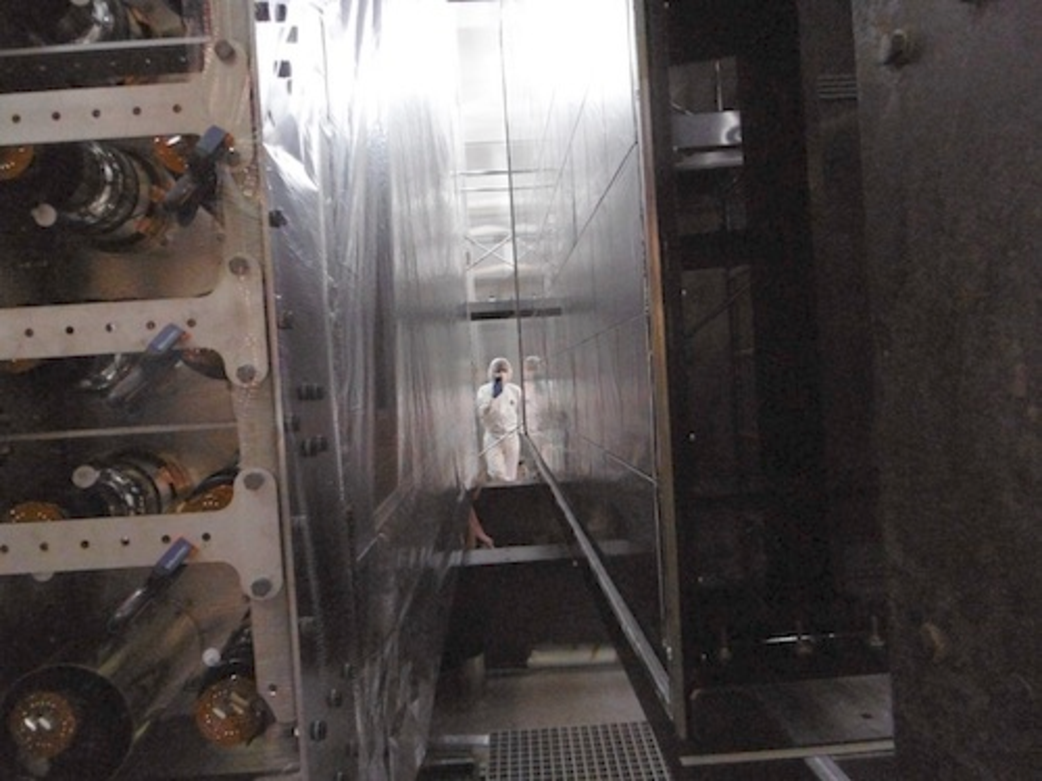
\includegraphics[width=0.7\textwidth]{SNdemonstrator/fig_SNdemonstrator/detector_closing.pdf}
\caption{Last picture of the SuperNEMO demonstrator before closing it, the $22$nd of November $2018$.
  The picture is taken from one side of the detector, facing the other side.
  We can distinguish on the right the front of one of the two calorimeter main walls, and on the left one of the two tracker chambers.
\label{fig:detector_closing}}
\end{figure}


\subsection{Detection principle}

The SuperNEMO demonstrator, in the manner of NEMO-$3$, combine tracking technology and calorimetry to record the full event kinematic, and measure the particle energies.
It is designed to search for the $\zeronu$ decay which, if observed, would prove the Majorana nature of the neutrino particle, opening the door of physics beyond the Standard Model, with huge implications in numerous physics research fields (in cosmology, for instance).
The SuperNEMO demonstrator is $6$~meters long, $3$~meters tall and $2$~meters deep.
It is the first of the $20$ modules that will make up the final detector.
This unique technology allows the experiment to characterise with a significant performance its own background, placing the detector in the ultra-low background category of experiments.

In Fig.~\ref{fig:demonstrator_scheme} is drawn a simplified scheme of the SuperNEMO demonstrator.
\begin{figure}[h!]
\centering
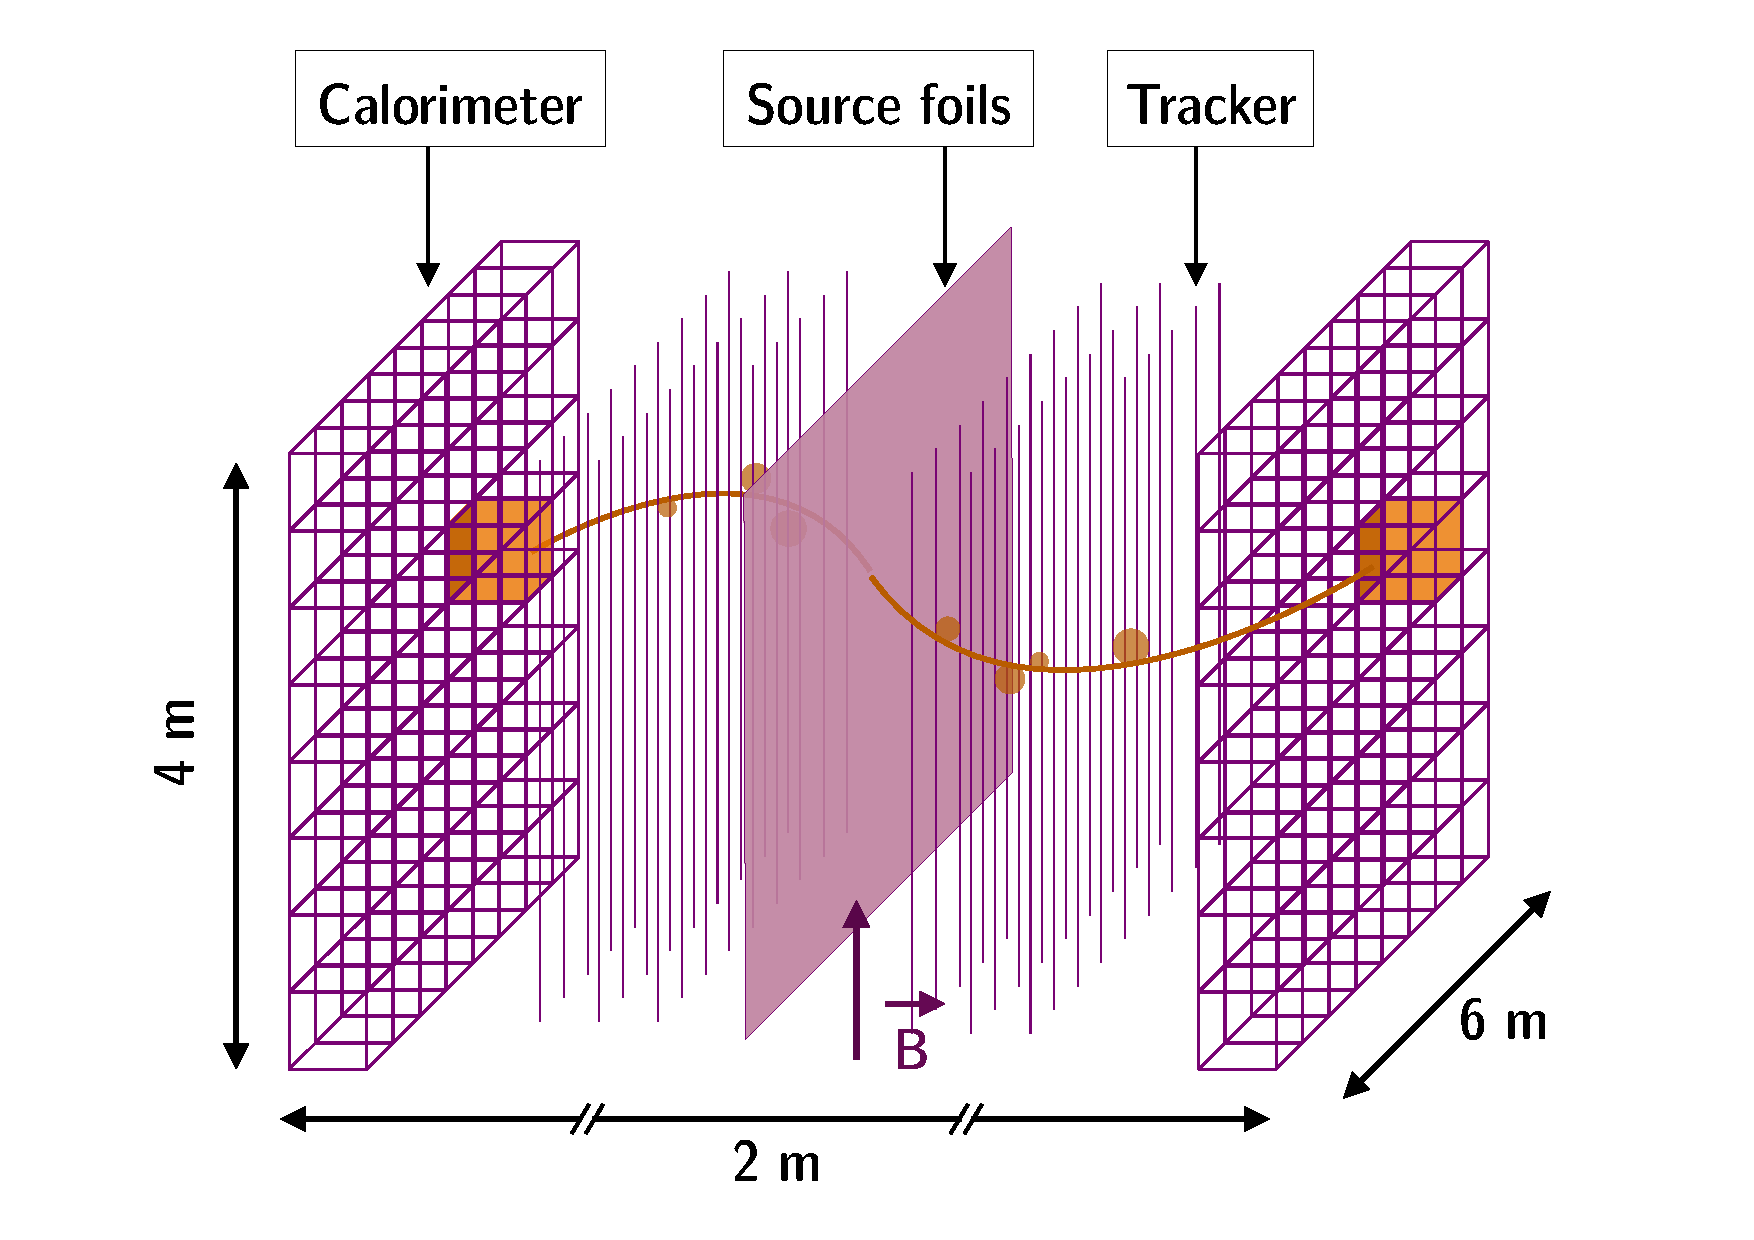
\includegraphics[width=1\textwidth]{SNdemonstrator/fig_SNdemonstrator/demonstrator_sheme.pdf}
\caption{Scheme of an open view of the SuperNEMO demonstrator (not to scale).
An example of emission from the source foils of two negatively charged particles is drawn.
\label{fig:demonstrator_scheme}}
\end{figure}
The isotope $\beta\beta$ emitter is distributed between ultra thin foils, at the centre of the detector.
The mass of isotopes studied with this technology is lower than for experiments using liquid scintillators or TPCs.
However, with the SuperNEMO design, the source is separated from the detector which allows to study any $\beta\beta$ isotope as long as it can be set up in thin foils, making this technology very interesting for the search of the $\zeronu$ decay.
We also schematise an emission of two negatively charged particles from the source, exiting in opposite directions.
The design of SuperNEMO as a layer of successive sub-detectors makes it possible to collect numerous information on the emitted particle.
When crossing the wire chamber, the charged particle ionises the gas, and the collected charge allows for the track reconstruction.
The detector is surrounded by a copper coil, delivering a magnetic field inside the wire chamber.
The trajectories of charged particles of few MeV are bent, allowing to discriminate electrons and positron of few MeV (which is not the case for muons and $\alpha$ particles).
Although the energy resolution and detection efficiency are modest compared to germanium or bolometer experiments, it is compensated by the powerful particle identification allowing to discriminate events coming from natural radioactivity decays.
Therefore, the tracking technology makes it possible to discriminate electrons from positrons (with the trajectory curvature), to identify $\gamma$ particles (corresponding to an energy deposit inside the calorimeter with no associated track), and to tag $\alpha$ particles (characterised by a short track inside the wire chamber).
The particle ends up in one of the scintillator blocks, where the collection of deposited charge by a photomultiplier tube (PMT) allows the incident particle energy measurement.
All electric signals are sent to the electronic boards where they are sampled and recorded for a later off-line analysis.

In addition to the search of the $\zeronu$ decay, the SuperNEMO technology is suitable for the search of other processes like double beta decays to exited states of the daughter nucleus that can be studied in dedicated channels (two-electrons and one/two gamma particles).
Thanks to the numerous topological informations brought by the successive sub-detectors, if the $\zeronu$ signal was observed, the SuperNEMO technology would also have the ability to discriminate between different hypothesised underlying mechanisms, allowing to investigate physics beyond the standard model.

In the following we describe in detail the successive layers of the SuperNEMO demonstrator, from the $\beta\beta$ emitter source foils to the electronic boards where the signal is sampled.


\subsection{The source foils}

\subsubsection*{Choice of isotope}

It exists numerous double beta emitters, coming from natural isotopes enriched in laboratory for physics research purposes.
The choice of the isotope is directed by several factors and experimental constraints.
Although this choice is specific to each detector, some constraint are common to all $\zeronu$ experiments.
\begin{itemize}
\item The energy transition $\Qbb$: the higher, the better.
Indeed, the ultimate background coming from natural radioactivity is the $\gamma$ of $2.615$~MeV emitted after the $\beta$ disintegration of \Tl.
Therefore, a high $\Qbb$ would help to guaranty the experiment to be background-free.
\item The phase space factor and the nuclear matrix element: as described in Sec.~\ref{sec:}, the $\zeronu$ half-life depends on these two parameters.
The higher they are, the more signal events are expected for a given data acquisition time.
\item The $\twonu$ half-life: this process represents an unavoidable background for the search of $\zeronu$.
Then, the higher the half-life of this process, the less $\twonu$ events are expected.
\item The natural abundance: The higher it is, the more we can produce substantial quantities of the enriched isotope.
\item Ease of enrichment: although it is not a measurable quantity as previous requirements, known purification techniques must be applicable to the isotope considered to reach high quantities of $\beta\beta$ emitter.
\end{itemize}
In Tab.~\ref{tab:bb_isotopes} are given some of the $\beta\beta$ emitter characteristics presented above [Pour Laurent: je ne suis pas totalement sûr de tous les chiffres, est-ce qu'on pourrait les vérifier ensemble?].
\begin{table}[h!]
\centering
\begin{tabular}{|c|c|c|c|c|c|}
\hline
Isotope & $Q_{\beta\beta}$ (MeV) & $G_{0\nu}$ ($10^{-15}$ y$^{-1}$) & $T^{2\nu}_{1/2}$ (y) & $\eta$ ($\%$) \\
\hline
\hline
$^{48}$Ca & $4.273$ & $24.81$ & $6.37\times 10^{19}$ & $0.187$ \\
$^{76}$Ge & $2.039$ & $2.363$ & $1.926\times 10^{21}$ & $7.8$ \\
$^{82}$Se & $2.995$ & $10.16$ & $9.6\times 10^{19}$ & $9.2$ \\
$^{96}$Zr & $3.350$ & $20.58$ & $2.35\times 10^{19}$ & $2.8$ \\
$^{100}$Mo & $3.035$ & $15.92$ & $6.93\times 10^{18}$ & $9.6$ \\
$^{116}$Cd & $2.809$ & $16.70$ & $2.8\times 10^{19}$ & $7.6$ \\
$^{130}$Te & $2.530$ & $14.22$ & $6.9\times 10^{20}$ & $34.5$ \\
$^{136}$Xe & $2.458$ & $14.58$ & $2.165\times 10^{21}$ & $8.9$ \\
$^{150}$Nd & $3.367$ & $63.03$ & $9.11\times 10^{18}$ & $5.6$ \\
\hline
\end{tabular}
\caption{$\beta\beta$ emitter used in current $\zeronu$ search.
$\Qbb$, phase space factor, $\twonu$ half-life and natural abundance are given.
\label{tab:bb_isotopes}}
\end{table}
\Se\ was chosen for SuperNEMO because of its high transition energy, and preferred to \Mo\ because of its higher $\twonu$ half-life.
Its nuclear phase space factor and natural abundance are satisfying and its enrichment does not pose any problem.

\subsubsection*{Source foils production}

The \Se\ isotope is enriched and purified by the ITEP laboratory in Russia.
Two purification techniques have been employed, given in Tab.~\ref{tab:Se_purification}.
\begin{table}[h!]
\centering
\begin{tabular}{|c|c|c|}
\hline
Enrichment technique & \Se\ quantity (kg) & Number of foils \\
\hline
\hline
Double distillation & $2$+$1.5$ & $11$+$8$\\
Reverse chromatography & $3$ & $15$\\
\hline
\end{tabular}
\caption{Different purification techniques and corresponding quantity of \Se\ isotope.
Two batches of \Se\ have been produced through double distillation.
\label{tab:Se_purification}}
\end{table}
Approximate isotope quantities are given for each technique.
A total of $6.23$~kg of \Se\ powder have been produced and purified.
After this purification step, the \Se\ is ground down to a fine powder ($50~\mu$m grains) and mixed with a radiopure glue.

To shape the \Se\ powder into the final SuperNEMO source foils, two distinct designs have been tested, one by ITEP and the other by the LAPP laboratory in Annecy (Fig.~\ref{fig:foils_design}).
\begin{itemize}
\item ITEP implemented the same technique as for NEMO-$3$ source foils, by smearing the \Se+glue mixture between two $12~\mu$m thick Mylar backing films, creating $3$~meters long foils.
The Mylar is perforated by irradiation, allowing the mixture to dry and better adhere to the film.
\item The LAPP team split up the foils in several pads: two Mylar sheets are heat welded together to host the several pads.
\end{itemize}
\begin{figure}[h!]
\centering
\begin{subfigure}[t]{0.49\textwidth}
\centering
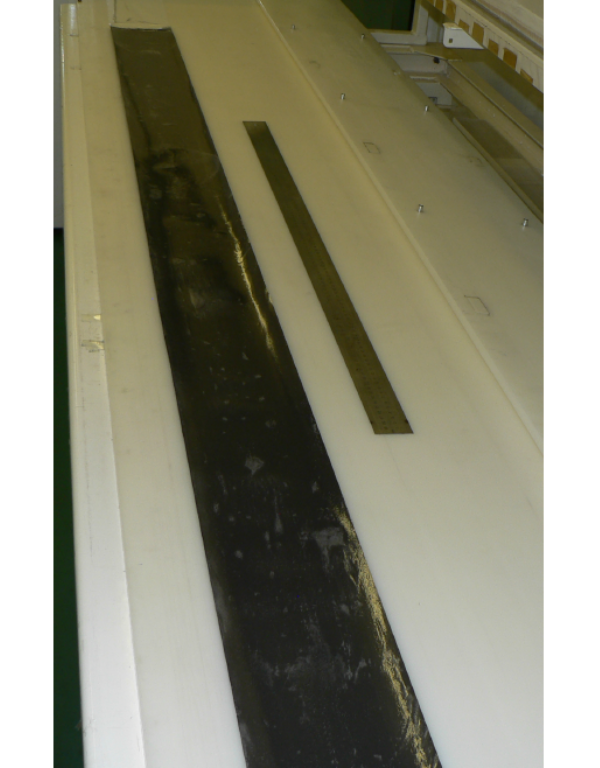
\includegraphics[width=0.9\textwidth]{SNdemonstrator/fig_SNdemonstrator/ITEP_source_foils.png}
\captionsetup{justification=centering}
\caption{ITEP style foils.
\label{subfig:ITEP_foils}}
\end{subfigure}
\hfill
\begin{subfigure}[t]{0.49\textwidth}
\centering
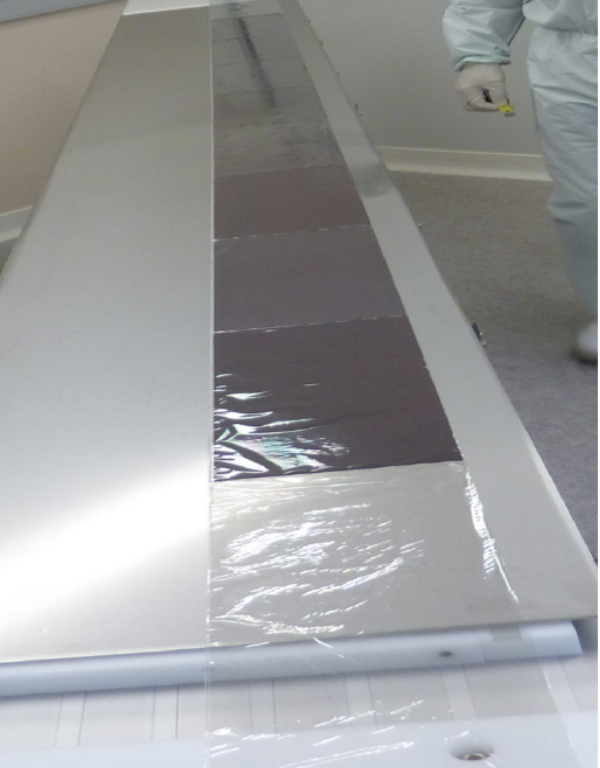
\includegraphics[width=0.9\textwidth]{SNdemonstrator/fig_SNdemonstrator/LAPP_source_foils.png}
\captionsetup{justification=centering}
\caption{LAPP style foils.
\label{subfig:LAPP_foils}}
\end{subfigure}
\caption{Two designs of source foils, ITEP (left) and LAPP (right).
\label{fig:foils_design}}
\end{figure}
The principal interest in designing the sources than thin is to maximise the chances of the electrons produced inside the source to escape it, to be detected by the successive sub-layers.
In addition, the collaboration made this design choice in order to leave the possibility of easy isotope change in the future.
Finally, the $6.23$~kg of \Se\ have been distributed into $34$ source foils measuring $135.5\times2700$~mm.
The thickness of the produced sources will be precisely measured by the collaboration and are expected to be [Combien ?].

\subsubsection*{Source foils installation}

Each strip was fasten to the source frame of $4.857$~meters long and $2.7$~meters large.
The source foils have been installed the $24$th September $2018$.
The original plan was to place the ITEP sources next to each other and to do the same for the LAPP sources.
Unfortunately, some of the sources had to be relocated because of source shape issues (in particular, some sources were in contact with the Bismuth calibration sources, discussed in Sec.~\ref{subsec:calib}).
The final position decided for the source foils are pictured in Fig.~\ref{fig:source_foils_installation}, where we can see the alternation of ITEP and LAPP sources.
\begin{figure}[h!]
\centering
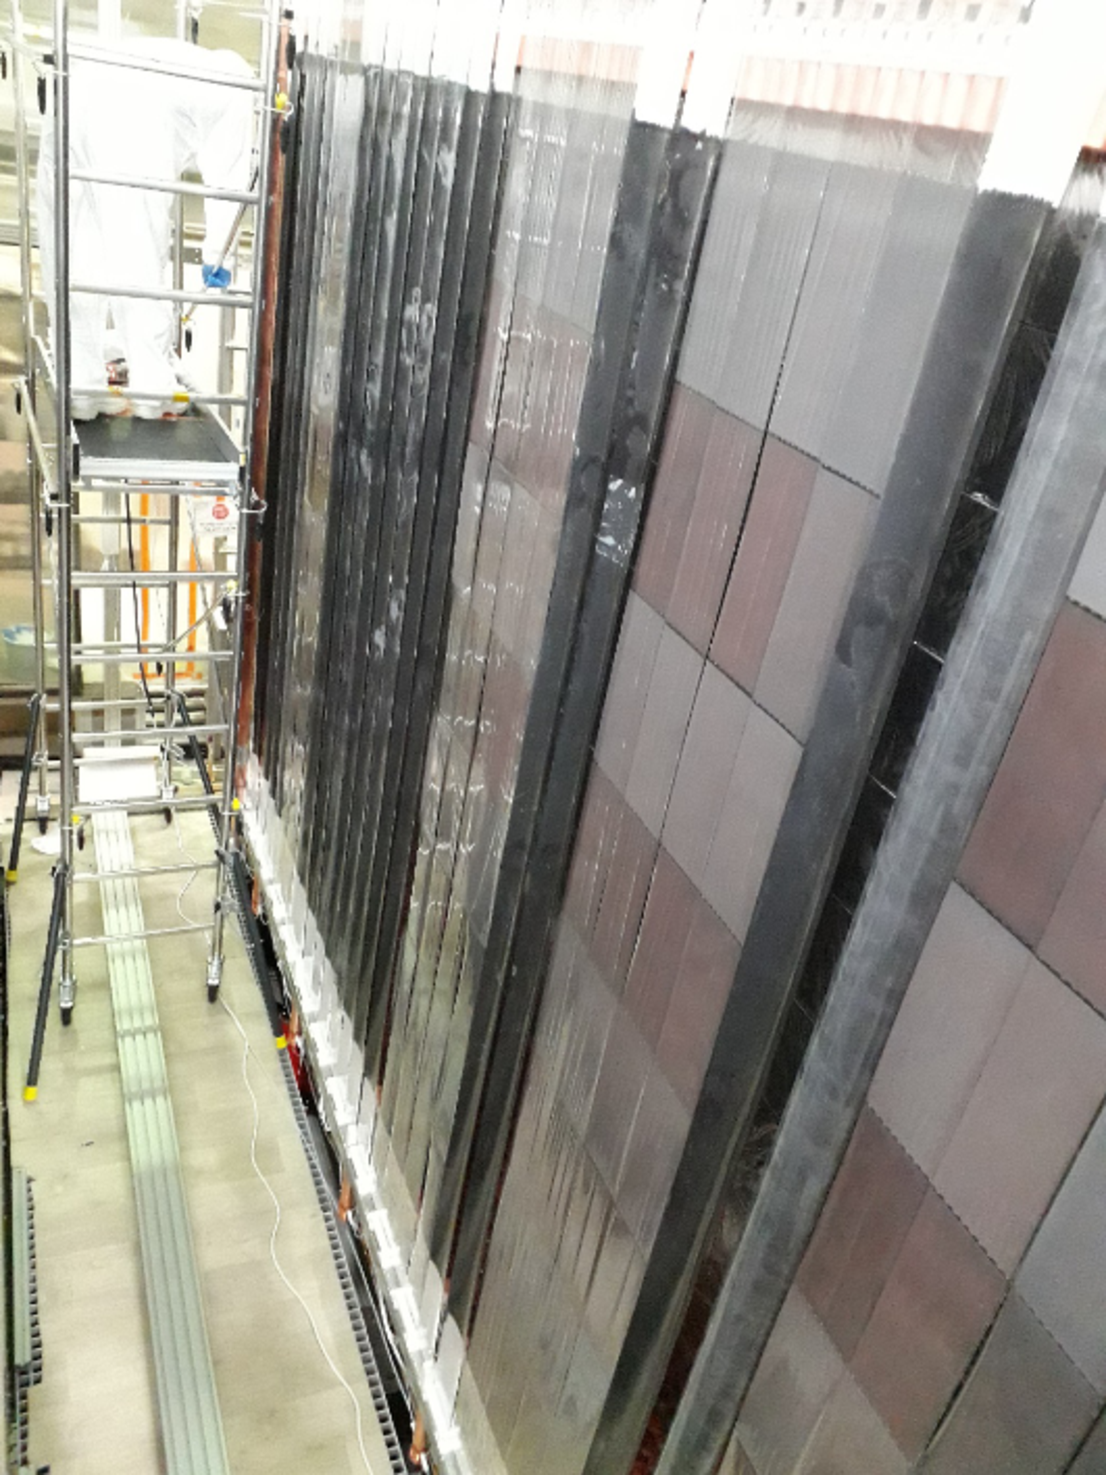
\includegraphics[width=0.7\textwidth]{SNdemonstrator/fig_SNdemonstrator/source_foils_final_position.pdf}
\caption{Final source foils position.
  The ITEP foils (one-piece long foils) and LAPP foils (divided in pads) are easily distinguishable.
\label{fig:source_foils_installation}}
\end{figure}
The final shape of the sources differs between the two types of sources: ITEP sources appear slightly curved on the image.
This probably happened when the sources were drying, because of the glue mixed with the \Se\ powder.
Each source curvature have been precisely measured using a laser, for a future integration in the reconstruction software.
I was part of the team that carried out the first curvature measurements after sources integration in Modane.

\begin{itemize}
\item Annexe position des sources
\item dire pq deux techniques : cf thèse Delphine (radiopurity)
\item mesure de radiopureté, BiPo ici ?
\end{itemize}

\subsection{The tracker}

The tracker is a detector aiming at measuring the charged particle three-dimensional trajectories, through their electromagnetic interaction with the gas filling the tracking chamber.
This sub-detector allows for efficient background rejection through the identification of particles, by making sure the event is composed of exactly two electrons.
The reconstruction of the vertices on the source makes it possible to identify highly contaminated areas, the so-called \emph{hot spots} of the experiment, and to reject them with appropriate cut-offs.
The SuperNEMO tracker is divided into two halves, one of each side of the source frame, to measure particles  coming out from the source in all possible directions.
It consists of a wire chamber filled with a gas mixture, operating in Geiger regime.

\subsubsection*{Geiger counters}

In Fig.~\ref{fig:geiger_avalanche} is schematised the basic operation principle of a Geiger cell.
\begin{figure}[h!]
\centering
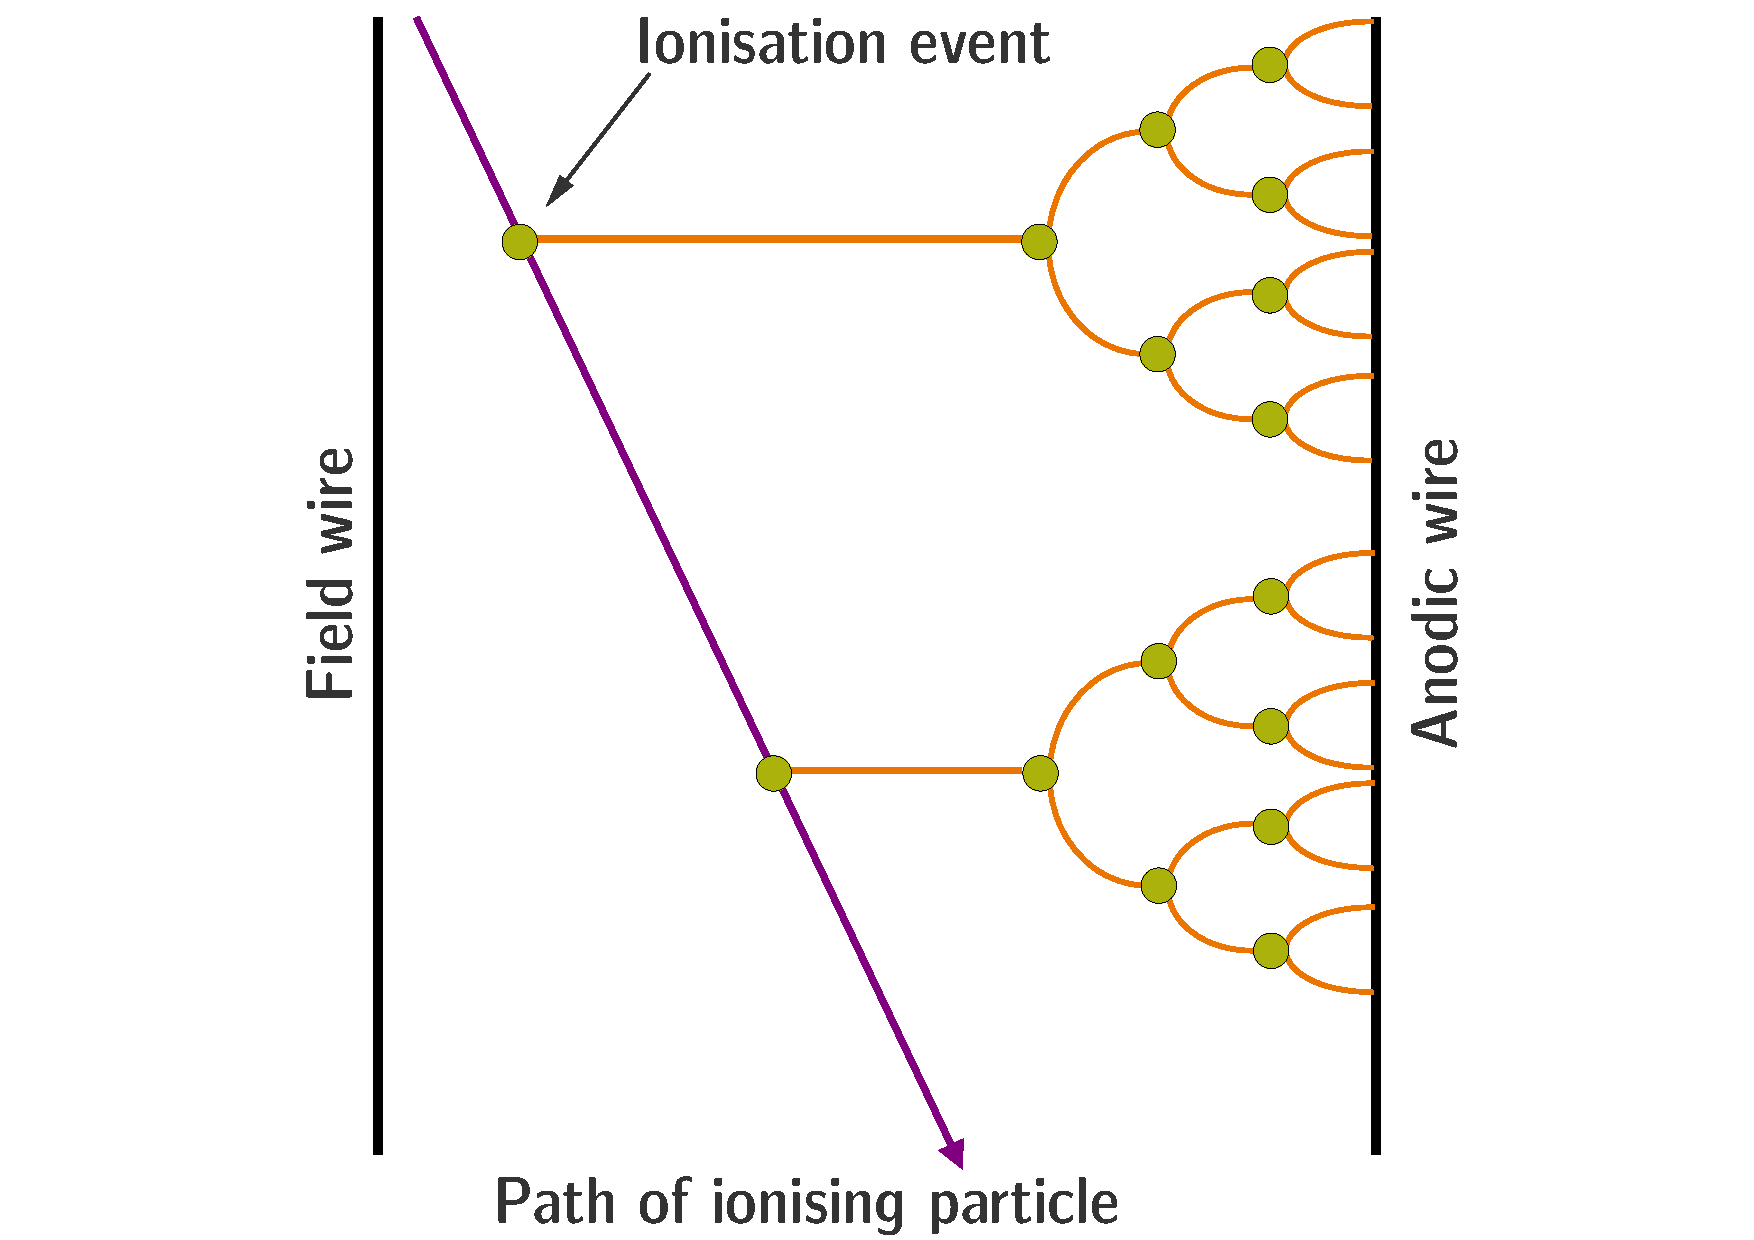
\includegraphics[width=0.7\textwidth]{SNdemonstrator/fig_SNdemonstrator/geiger_avalanche.pdf}
\caption{The principle of a Geiger cell illustrated with the anode and one cathode.
\label{fig:geiger_avalanche}}
\end{figure}
When a particle goes through the the gas in which the Geiger cell is immersed, it ionises it all along its path, creating positive charges on one hand (heavy ions) and negative on the other hand (electrons).
As a high electric potential is applied between the anode and cathode, the freed electrons drift towards the negative electrode, and the ions towards the positive one.
The electric field is as strong as the freed electrons are even accelerated, in turn ionising the gas, creating electronic avalanches until the ground wire is reached.
The Geiger mode is obtained when the avalanches created by the electrons are saturated: increasing the voltage does not increase the collected charge.
This is the so-called \emph{Geiger plateau}, which provides a very high detection efficiency ($>99$\%).


\subsubsection*{SuperNEMO Geiger cells}

A minimal amount of material is required inside the tracker chambers, for the particles to cross freely the detector, with limited energy losses (du to multiple scatterings on the wires for instance).
However, a minimal distance between the tracker wires is required in order to collect efficiently the charges coming from gas ionisation.
Taking into account the tracker spacial resolution needs and the constraints on gas mixture composition, the decision was made to design Geiger cells as in Fig;~\ref{fig:SN_geiger_cell}, with one central anode wire (stainless steel, $40\mu$~m in diameter) and $12$ surrounding cathodes wires (stainless steel, $50\mu$~m in diameter).
\begin{figure}[h!]
\centering
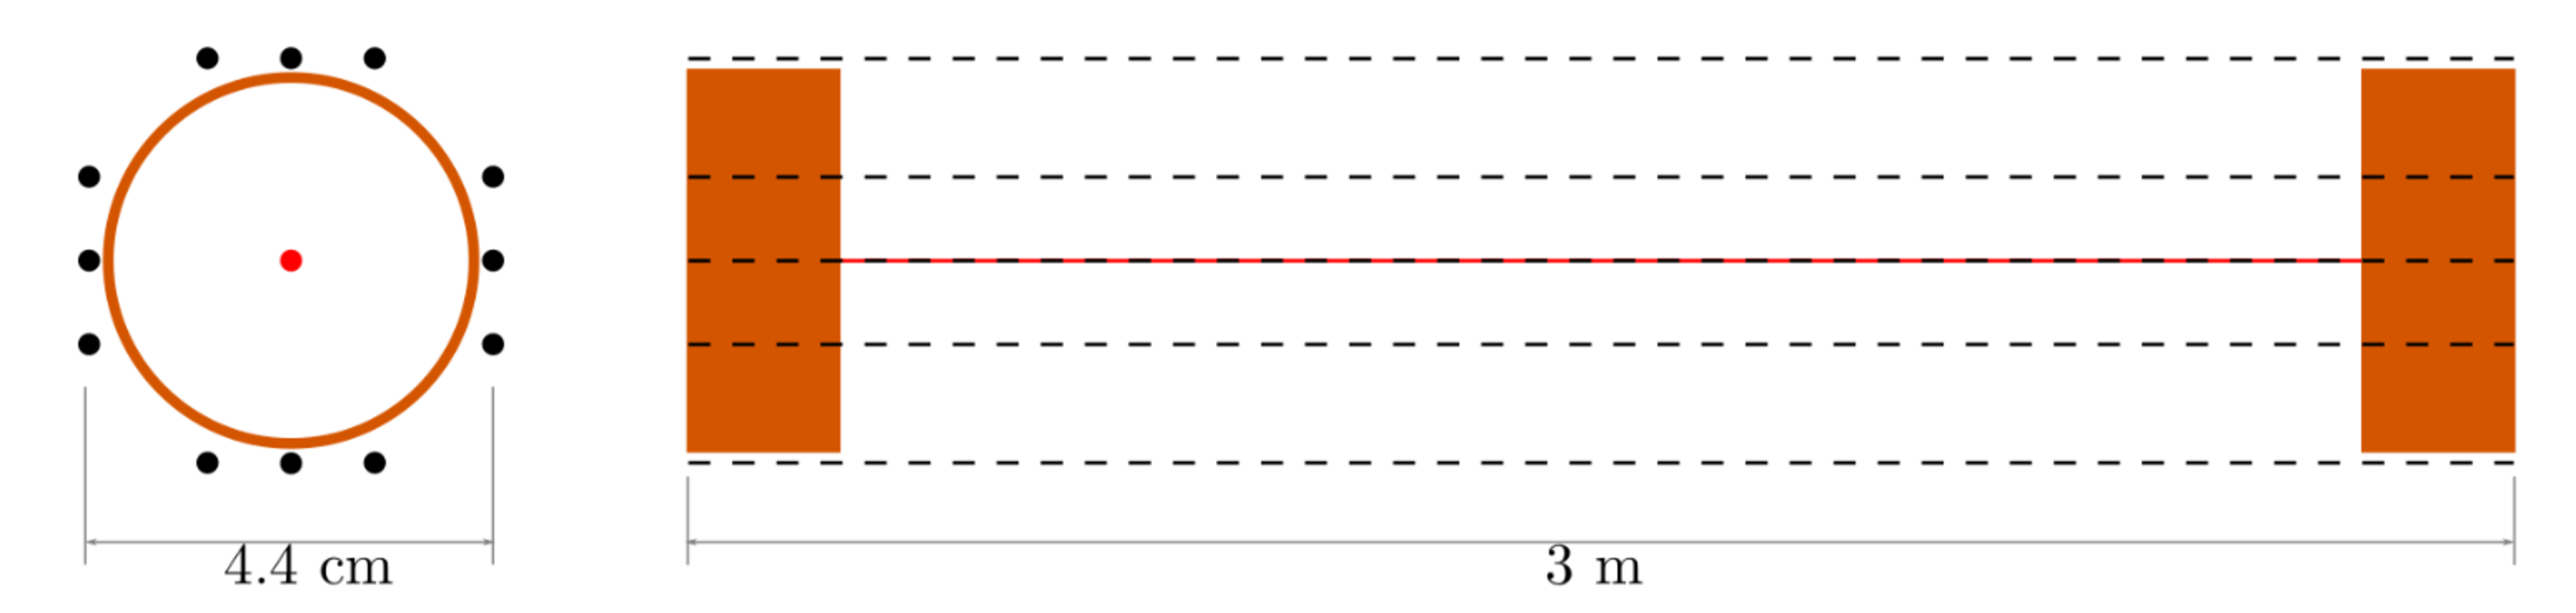
\includegraphics[width=1\textwidth]{SNdemonstrator/fig_SNdemonstrator/geiger_cell.pdf}
\caption{Sketch of a SuperNEMO Geiger cell, in transverse view (left) and side view (right, the sketch is rotated of $90^{\circ}$ as the Geiger cells are vertical in the SuperNEMO demonstrator).
  The anode central anode is represented at the centre in red.
  Cathode wires, in black, surround it to form $4.4$~cm large and $3$~m long Geiger cells.
  On the right the copped rings are also represented by orange stripes on each side of the wires.
\label{fig:SN_geiger_cell}}
\end{figure}
Each cell has a large diameter of $\sim~4$~cm.[ mesure à vérifier]
Two copper rings, of $4$~cm diameter and $4$~cm long, are placed on both ends of each cell, allowing the cessation of the avalanches. [si on ne met pas les copper rings, qu'est-ce que ça change ? Et comment est-ce que ces pièces arrêtent l'avalanche ?]
In total, the tracker chamber is composed of $2034$ Geiger cells of $3$~m long, divided in a $9\times113$ layer configuration, parallel to the source foils.
Each cell can measure the radial distance (the distance of the particle from the anode) and the longitudinal distance (the position along the cell axis).
The latter is obtained with the time needed for these avalanches to reach both ends of the cell.
In the SuperNEMO operating conditions, the avalanche is expected to spread through a cell in about $50~\mu$s.

As we said, the behaviour of a Geiger cell depends on the voltage applied.
For the SuperNEMO cells, the Geiger plateau is located around $1800$~V.
However, the exact voltage to be applied to each cell depends on their individual properties, and will have to be determined and set up after the tracker commissioning phase.


\subsubsection*{Gas mixture}

The gas mixture is decisive for the wire chamber operation.
For the SuperNEMO chambers, it is composed as follows:
\begin{itemize}
\item Helium is the main component of the gas mixture, which is ionised by incident radiations. As an inert gas, it does not react with the detector sensitive parts.
\item Argon ($1$\%) enhances the propagation of avalanches along the anode wires thanks to its lower ionisation energy.
\item Ethanol ($4$\%) is used as a quenching agent, stopping the successive discharges without external assistance.
\end{itemize}
This gas is maintained at low pressure, to guarantee a low $Z$ medium in order to minimise the energy losses occurring through multiple scattering.
[A discuter avec Laurent, car cette histoire de low pressure c'est quelque chose que j'ai vu aussi dans le manuscrit de Steven, mais on parle de surpression...]

\subsubsection*{Tracker installation}

Each tracker side is divided in two C-sections (named in this way according to the C-shape of each section) assembled in the University of Manchester.
They were delivered individually and integrated in Modane to form the two tracker chambers.
In Fig.~\ref{fig:me_tracker} is given a picture of the tracker after its integration to the detector.
\begin{figure}[h!]
\centering
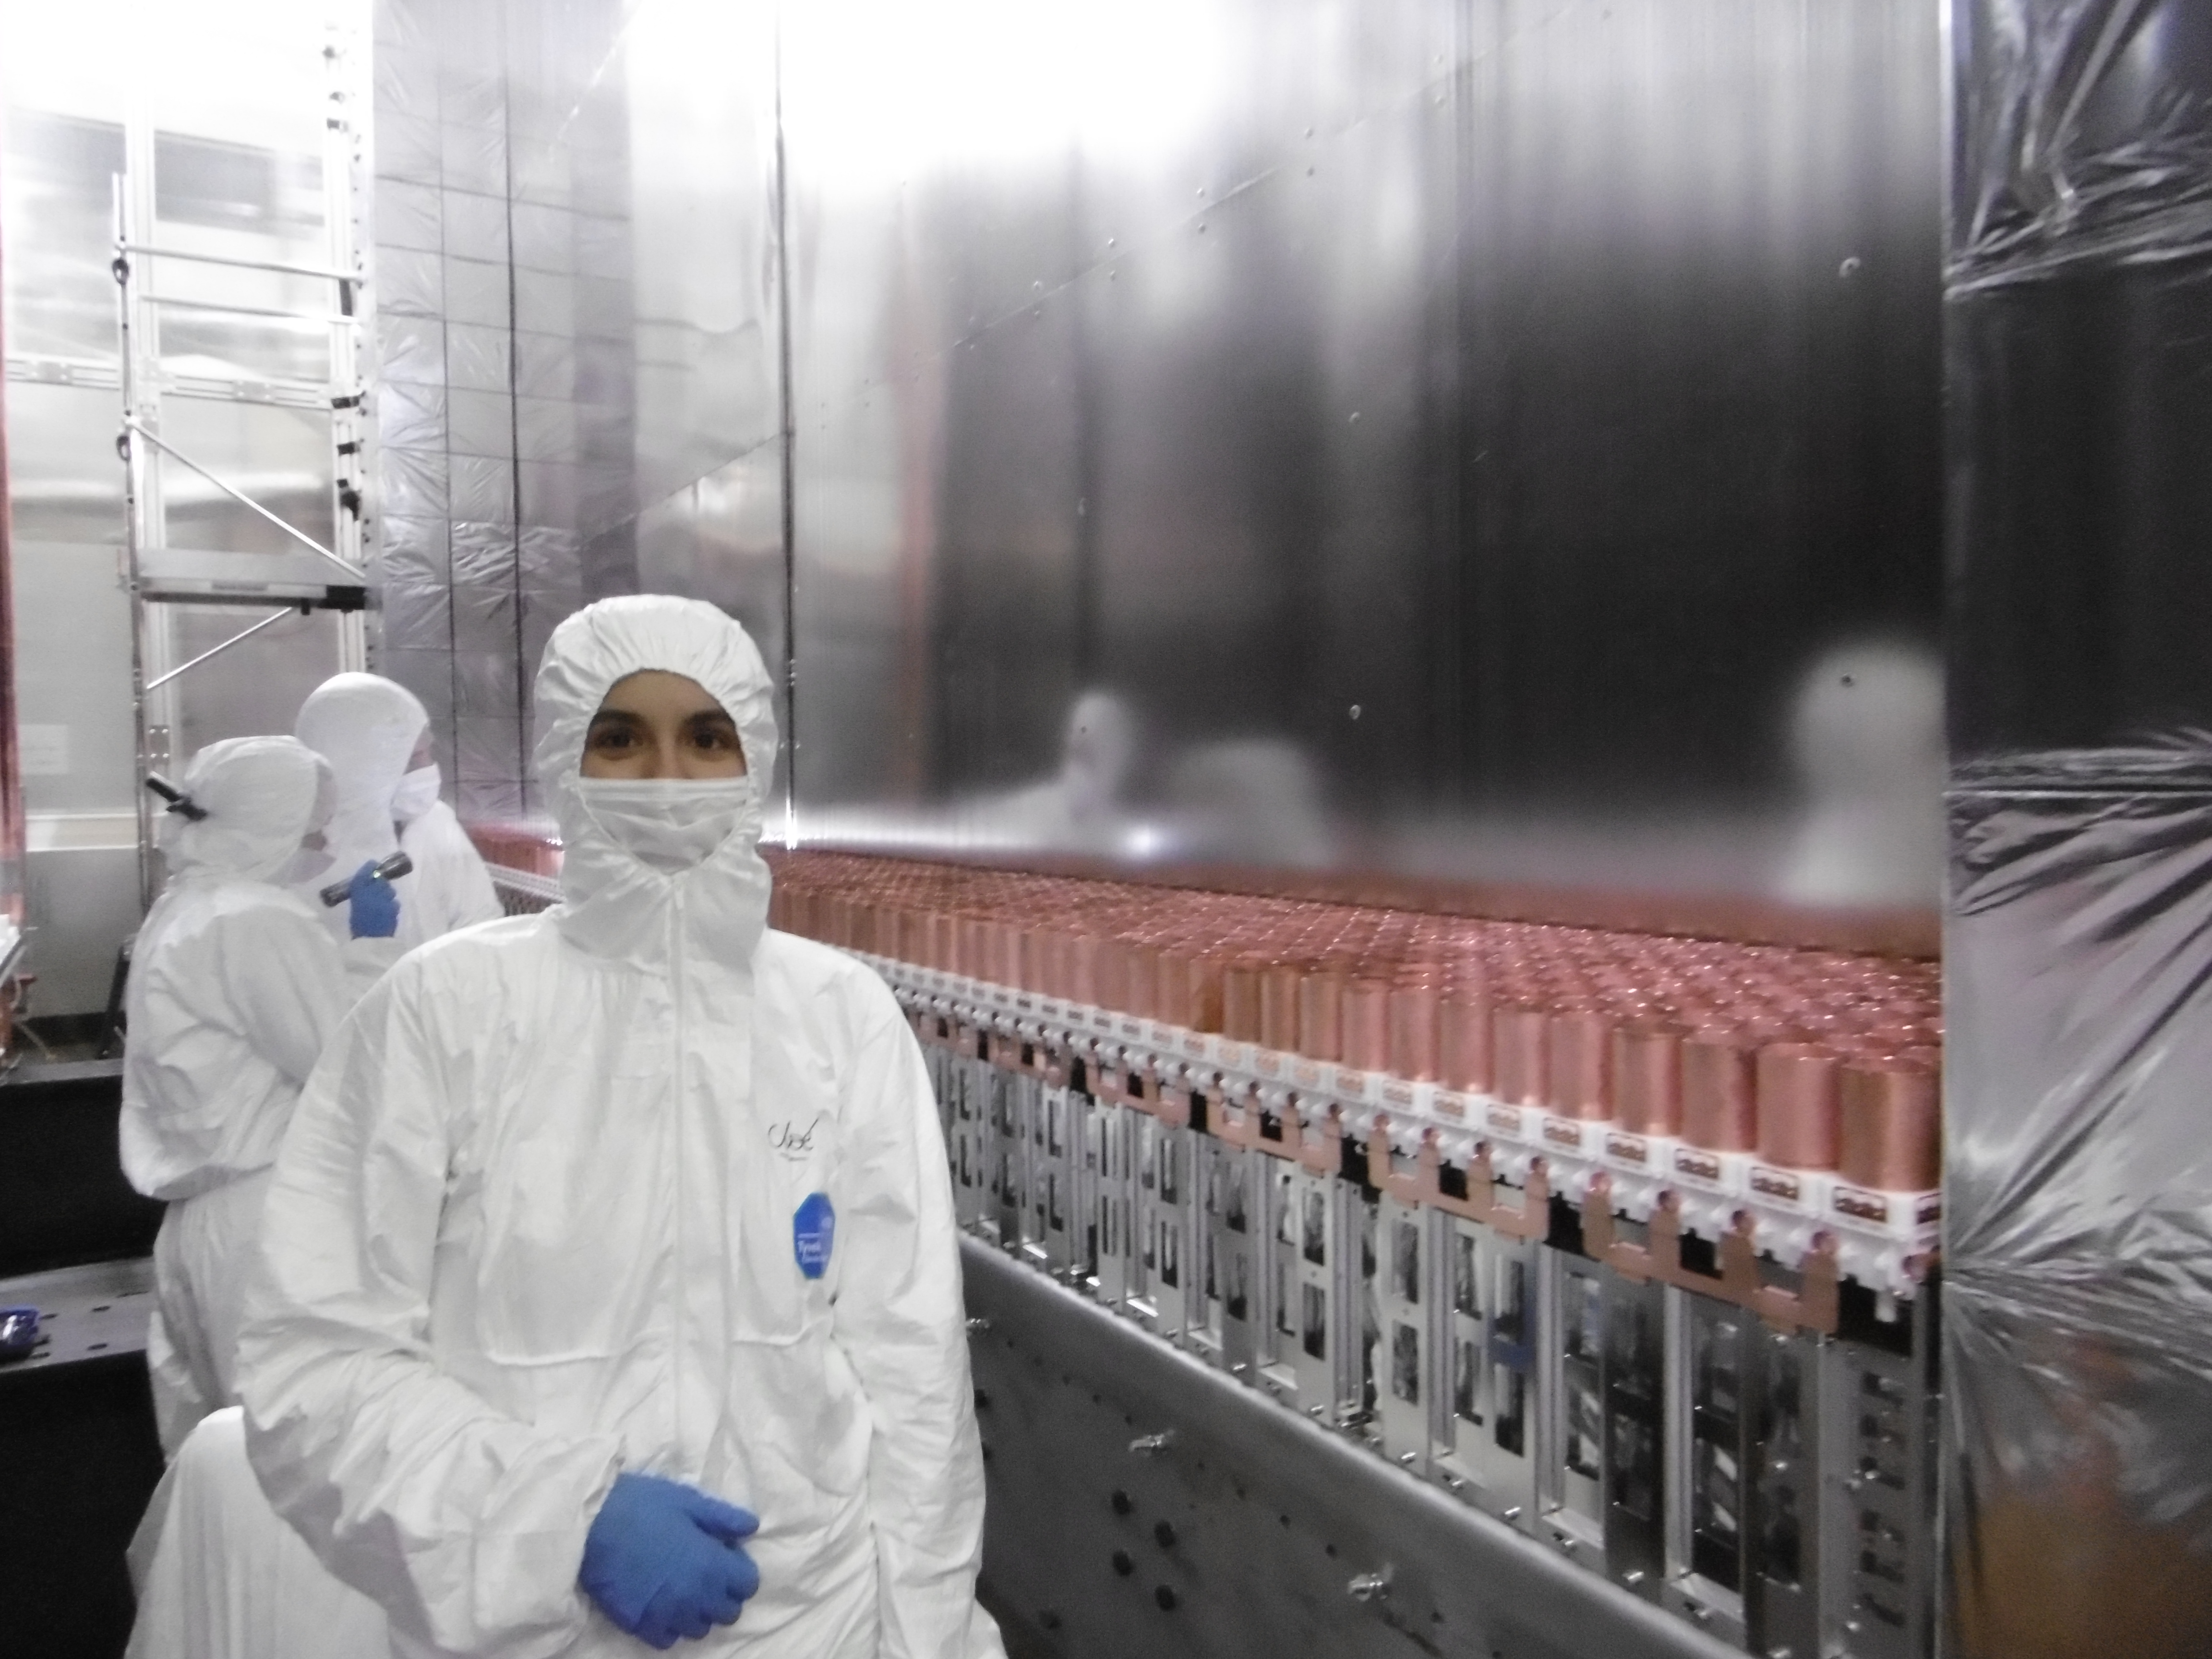
\includegraphics[width=0.9\textwidth]{SNdemonstrator/fig_SNdemonstrator/tracker_selfie.jpg}
\caption{Inside view of the tracker (with me standing in the foreground), before detector closing, on the day of the wire check, looking for possible broken wires at the base of the copper rings.
\label{fig:me_tracker}}
\end{figure}
The bottom copper rings are noticeable and indicate the presence of the Geiger cells whose wires are too thin to be visible on the picture.
After installation, some meticulous work were achieved to remove few wires damaged during transport.

\subsubsection*{Gas sealing}

Once the tracker was integrated into the detector, a huge effort was achieved by the entire collaboration to seal it.
Indeed, the tracker has to be under constant gas over-pressure, mainly to prevent the Radon-contaminated gas from entering the detector.
As a thesis student in the collaboration, I had the opportunity to participate in much of this work.

\begin{itemize}
\item étanchéïté notamment pour Helium et surpression (participé aussi)
\item identification hotspots
\item donner résolution spaciales et temporelles
\item pourquoi les pads du LAPP ont une couleur différente ?
\end{itemize}

\subsection{The calorimeter}
\label{subsec:SN_calo}

\begin{itemize}
\item Bien détailler cette partie puisque on a fait le commissioning
\item On mesure l'énérgie des particules car c'est la variable discriminante 2nu/0nu
\item MW, gamma-V et XW (nb de calo dans chaque catégorie)
\item scintillator (polystyrene, POPOP...) peut être aller voir dans le chapitre Cobalt ce que j'ai écrit et qui peut être déplacé ici. Décrire toute la chaine d'interaction
\item PM, pareil décrire en détail le principe de détection
\item Teflon et Mylar
\item energy resolution
\end{itemize}

\subsection{The magnetic coil and the shieldings}

\label{sec:magnetic_field}

It is, however, not high enough to impact significantly neither the few muons nor the $\alpha$ particles expected to be detected by the tracker.
Due to their much higher momenta, they will instead leave straight tracks in the wire chamber.

\subsection{Calibration strategy}
\label{subsec:calib}

\subsection{Control Monitoring system}

\subsection{Electronics}
\begin{itemize}
\item The electronics commissioning has begun in June 2018 at Manchester.
\end{itemize}


\subsection{Detector cabling}

\section{Backgrounds}
\label{sec:SNbkg}

\begin{itemize}
\item radiopurity
\item section sur BiPo (voir artcile sur site SuperNEMO.org)
\end{itemize}

\subsection{Internal background}
\label{subsec:SNbkg_internal}

Trace quantities of naturally-occurring radioactive isotopes can occasionally produce two-electron events and thus can mimic $\beta\beta$-decay events.
The largest contributions come from isotopes of decay chains of $^{238}$U, $^{232}$Th and $^{40}$K, which disintegration occur inside the source foils, as well as inside the tracking volume.

Décire la contamination mesurée des sources, et du radon dans la partie suivante

\begin{figure}[!h]
\centering
\begin{subfigure}[t]{0.32\textwidth}
  \centering
  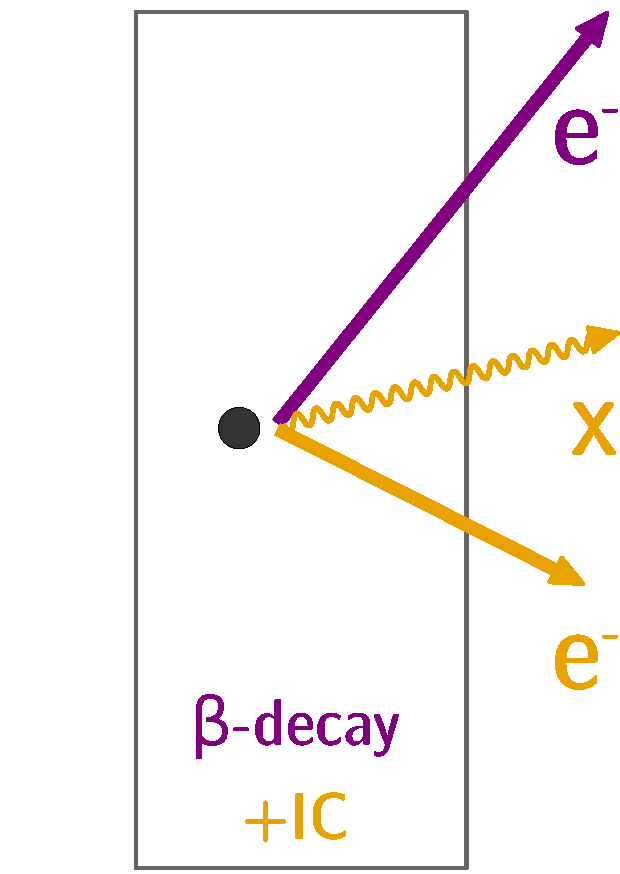
\includegraphics[width=0.82\textwidth]{SNdemonstrator/fig_SNdemonstrator/internal_contamination_IC.pdf}
  \captionsetup{justification=justified}
  \caption{
    \label{subfig:cont_Pint_eff}}
\end{subfigure}
\hfill
\begin{subfigure}[t]{0.32\textwidth}
  \centering
  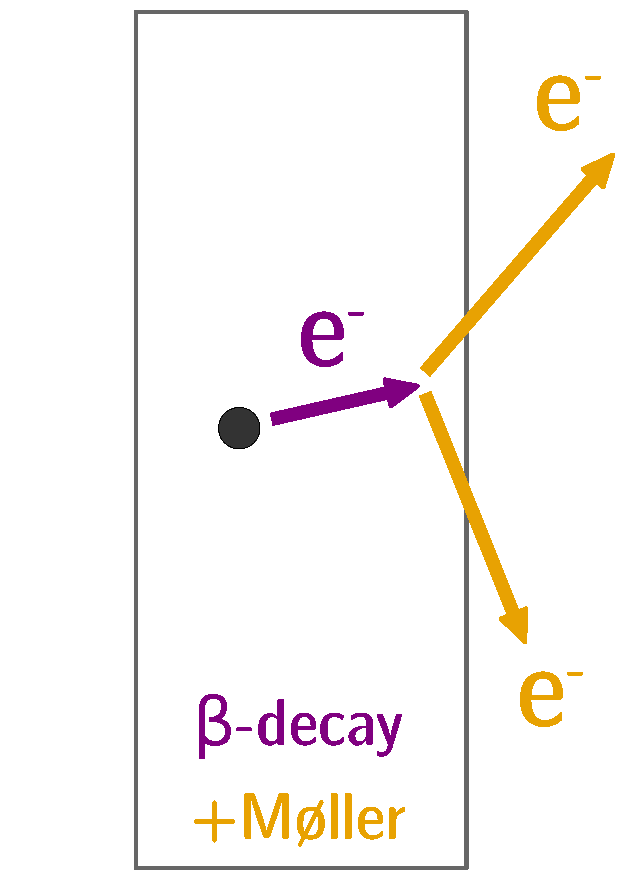
\includegraphics[width=0.82\textwidth]{SNdemonstrator/fig_SNdemonstrator/internal_contamination_moller.pdf}
  \captionsetup{justification=justified}
  \caption{
    \label{subfig:cont_Pint_ROI}}
\end{subfigure}
\hfill
\begin{subfigure}[t]{0.32\textwidth}
  \centering
  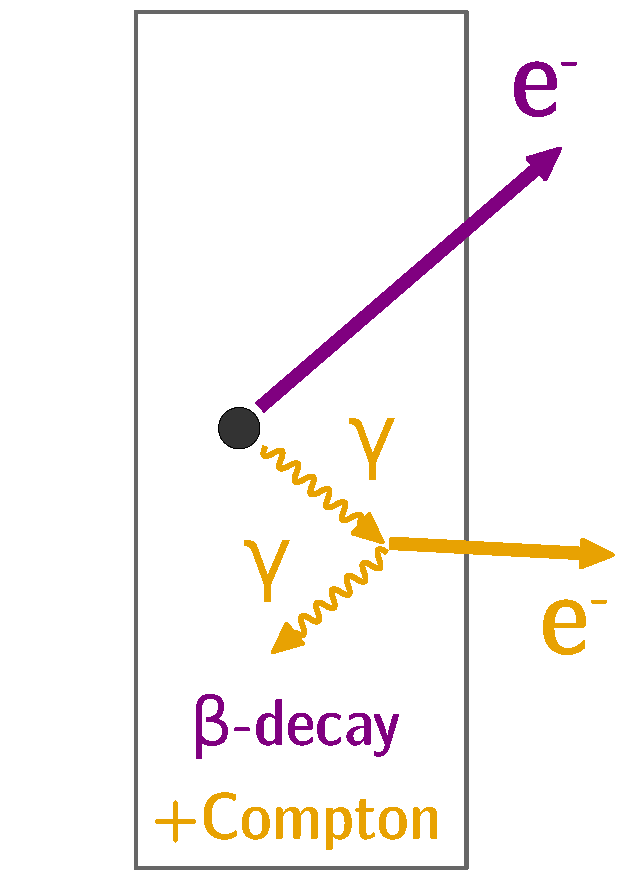
\includegraphics[width=0.82\textwidth]{SNdemonstrator/fig_SNdemonstrator/internal_contamination_compton.pdf}
  \captionsetup{justification=justified}
  \caption{
    \label{subfig:cont_Pint_ROI}}
\end{subfigure}
\caption{(a) $\beta$ decay + internal conversion: radioactive nucleus performs a $\beta$ decay, then an electron is emitted after internal conversion of photon
    (b) $\beta$ decay + M\o{}ller:
    (c) $\beta$ decay + Compton diffusion: radioactive nucleus $\beta$ decays to an excited state, then the photon perfoms a Compton diffusion.
  \label{fig:internal_contamination}}
\end{figure}

\subsubsection{Measurement of \Tl\ in the one electron and $n\gamma$ channel}

The \Tl\ contamination inside the source foils is one of the main backgrounds for the neutrinoless double beta decay, with the internal \Bi, as well as the Radon gas in the tracker.
One of the key features of the SuperNEMO demonstrator remain its ability to measure its own background in dedicated channels, which are independent from the main signal channels.

As explained before, \Tl\ emits one electron and between $1$ and $3$ $\gamma$’s.
Consequently, the $1e1\gamma$, $1e2\gamma$ and $1e3\gamma$ channels can be used to discriminate internal \Tl\ events, and measure the activity of the source.
However, since the particles share the same fixed energy, the more particles there are, the less energy they will carry.
It is therefore less likely for three $\gamma$ to be detected in a short time range, since the half-life times of these levels are very small and the gamma rays pass through the detector.
A significant contribution to the $1e1\gamma$ and $1e2\gamma$ channels is also expected from other radio contaminants, like \Bi, and from radon events.

Specified contamination levels have been established in order to achieve the $\zeronu$ half-life target of $\sim 1\times 10^{26}$~years for the final detector.
The \Se\ demonstrator source is segmented in $34$ foils, whose production was the responsibility of different laboratories (Dubna, LAPP and Tomsk).
The sources have undergone different purification treatments, in order to investigate new techniques, and to compare them with those of NEMO-$3$.
After the sources production and purification, preliminary measurements have been performed with the BiPo-$3$ detector to determine the actual \Tl\ and \Bi\ contamination levels inside the foils~\cite{internal:bipo}.
The level of radon emissions inside the tracker was also measured by the collaboration, for each of the four sections of the chamber, using a concentration line.
We summarise all these contamination levels in Tab.~\ref{tab:real_target_act}, and give a comparison with the detector initial specifications.
\begin{table}[h!]
  \centering
  \begin{tabular}{|c|c|c|}
    \hline
    & Specified activities & Measured activities \\
    \hline\hline
    \Tl  & $2\,\mu$Bq.kg$^{-1}$ & $54\,\mu$Bq.kg$^{-1}$ [$26$~-~$102$] \\
    \Bi  & $10\,\mu$Bq.kg$^{-1}$ & $<290\,\mu$Bq.kg$^{-1}$ \\
    \Rn  & $0.15$ mBq.m$^{-3}$ & $0.15\pm 0.02$ mBq.m$^{-3}$ \\
    \hline
  \end{tabular}
  \caption{Measured and specified activities for the SuperNEMO demonstrator.
    The \Rn\ tracker contamination is measured with a concentration line~\cite{conf:radon2017}, extrapolated with a $2$~m$^{3}$/h flow rate.
    The limit on \Bi\ contamination is provided by BiPo measurements for a $90\%$ CL~\cite{internal:bipo}.
    \label{tab:real_target_act}}
\end{table}
The targeted \Tl\ level is not reached, being almost $27$ times higher than expected, and $3.0\times 10^{4}$ internal Thallium events are expected in $2.5$ years.
Nevertheless, on average, the activity of the sources was improved by a factor of $2$ compared to the $^{100}$Mo sources of NEMO-$3$.
In addition, valuable information has been accumulated on the different production techniques, which are of great importance for the final detector construction.
In particular, the two best \Tl\ sources activities were reached by inverse chromatography, reaching a $20\pm10~\mu$Bq/kg level, an improvement by a factor $5$ compared to NEMO-$3$.
This encourages for further investigations in this direction.
The sensitivity of BiPo detector only allowed to give an upper limit on the level of internal \Bi\ (an activity of $290~\mu$Bq/kg would correspond to $1.6\times~10^{5}$ internal Bismuth events in $2.5$ years).
Precise measurements are expected from the demonstrator calibration.
Radon emissions from the tracker were also measured, and extrapolated with an air flow rate of $2$~m$^{3}$/h inside the chamber, showing the targeted level of $0.15$ mBq.m$^{-3}$ was reached.


\subsection{External background}
\label{subsec:SNexternal_bkg}

Radon:\\
Radon is a noble gas which occurs as an indirect decay product of uranium and thorium.
Due to its chemical properties, radon has a long diffusion length in solids, making it difficult to remove.
Radon contaminations inside the tracker volume is a major background to the rare event experiments such as SuperNEMO.
Simulations show that, to achieve the designed sensitivity, the level of radon must not exceed $0.15$ mBq/m$^{3}$ since its decay daughter \Bi, $\Qbb= 3.2$ MeV can mimic a $\zeronu$ event.
Radon concentration measurements inside the demonstrator tracker have been performed by the SuperNEMO collaboration, revealing an activity of $0.15\pm0.02$ mBq/m$^{3}$, through the combination of an anti-radon tent and an air-flushing method.

%%Repris d'un article -> a changer:
They are outgased in the air from the rock walls of the experimental hall and can enter the detector either through tiny gaps between sectors or through gas pipe joints.
The progeny of radon and thoron produces $\gamma$-rays and $\beta$ decays accompanied by internal conversion (IC), Møller or Compton scattering.


\subsection{Background reduction}

\subsubsection{The underground laboratory}

\subsubsection{External shield}


\section{The SuperNEMO software}
\label{sec:SNsoftware}
\subsection{Simulation}

As described in Sec.~\ref{sec:SNsoftware} of Chapter~\ref{ch:detector}, the SuperNEMO collaboration developed its own simulation, reconstruction and analysis environment.
The Falaise software, specifically designed by and for the SuperNEMO collaboration, holds the \verb!C++! library for the event reconstruction and analysis of simulated and real data.
Especially, it contains the geometry, the detector material, the event data model, the reconstruction algorithms and the data analysis.
Finally, the SNFee software is a tool package for the configuration, control and monitoring of the SuperNEMO front-end electronics.

\subsection{Reconstruction}

Particle identification with detector scheme

\subsection{Monte-Carlo simulations}

\subsection{Analysis chain}


\subsection{Modifications of simulation software}



\section{Analysis tools}

\subsection{Internal probability}
\label{subsec:internal_prob}

Internal probability is a mathematical tool used to quantify the probability that two particles were emitted simultaneously and at the same location in the source foils.
This tool is based on the particle Time-Of-Flight computation.
%and this measurement can only be performed if both particles have at least one associated calorimeter hit, and that one of them is charged (a vertex is needed to formulate a hypothesis.)
Firstly, we define, for two particles, the internal $\chi^{2}$
\begin{equation}
  \chi^{2}_{int}=\frac{((t^{exp}_{1} - t^{th}_{1}) - (t^{exp}_{2} - t^{th}_{2}))^{2}}{\sigma_{tot}^{2}}\,.
  \label{eq:int_chi2}
\end{equation}
$t^{th}_{i}$ is the theoretical time of arrival of the particle $i$ inside the calorimeter, $t^{exp}_{i}$ the arrival time experimentally measured, c is the speed of light, and $\sigma_{tot}$ is the quadratic sum of all uncertainties.
The theoretical time, is defined as
\begin{equation}
  t^{th}_{i}=\frac{L_{i}}{\beta_{i}\,c}\,,
  \label{eq:th_time}
\end{equation}
where $L_{i}$ is the reconstructed track length, and $\beta_{i}$ corresponds to
\begin{equation}
  \beta_{i}=\frac{\sqrt{E_{i}(E_{i} + 2m_{i})}}{E_{i} + m_{i}}\,,
  \label{eq:beta_i}
\end{equation}
$E_{i}$ being the energy of the particle and $m_{i}$ its mass.
The total uncertainty, $\sigma_{tot}$, is defined as
\begin{equation}
  \sigma_{tot}=\sqrt{\sigma_{t_{1}}^{2}+\sigma_{t_{2}}^{2}+\sigma_{\beta_{2}}^{2}+\sigma_{\beta_{1}}^{2}+\sigma_{l_{1}}^{2}+\sigma_{l_{2}}^{2}} \,.
  \label{eq:sigma_tot}
\end{equation}
We compare the experimental time difference to the theoretical time difference, to see if it can be explained only by the difference in track lengths.
If it is compatible, which means of the order of the experimental uncertainties, the associated $\chi^{2}$ will be low i.e. close to $1$ or lower.

\paragraph{The uncertainty $\sigma_{t}$ on the time measurement}
This term is directly related to the phenomenon of absorption and re-emission of scintillation photons detailed in Chapter~\ref{ch:commissioning}.
It is defined as
\begin{equation}
  \sigma_{t}=\sqrt{\dfrac{\tau_{\text{SC}}^{2}+\left(\dfrac{\text{FWHM}_{\text{TTS}}}{2\sqrt{2\ln{2}}}\right)^{2}}{\text{N}_\text{PE}}}\,,
  \label{eq:sigma_t}
\end{equation}
where $\tau_{\text{SC}}$ is the scintillator characteristic time, due to the scintillator de-excitation time: it corresponds to the time emission of the scintillation photon responsible for the creation of the photoelectron on the photocathode.
$\text{FWHM}_{\text{TTS}}$ is the temporal dispersion linked to the photomultiplier: the transit time of the photoelectrons inside the photomultiplier can evolve, according to its point of creation on the photocathode.
This transit time is unique for each photomultiplier, and has to be characterise experimentally.
For the SuperNEMO scintillators, $\tau_{\text{SC}}=2.5$~ns~\cite{ref} and $\text{FWHM}_{\text{TTS}}=2.25$~ns~\cite{ref}.
$\text{N}_\text{PE}$ is the number of photo-electrons emitted after a particle has deposited all its energy $E$ in the scintillator:
\begin{equation}
  \text{N}_\text{PE} = E\times \left(\frac{2\sqrt{2\ln 2}}{\text{FWHM}_{\text{E}}}\right)^{2}\,,
\end{equation}
where $\text{FWHM}_{\text{E}}$ is the energy resolution of the PM, $8~\%$ at $1$~MeV for the SuperNEMO calorimeter.
Therefore, for a particle of $1$~MeV depositing all its energy inside a scintillator, $\text{N}_\text{PE}\sim 866$ photo-electrons are emitted, an improvement of ?~\% compared with NEMO-$3$.
Finally, the uncertainty $\sigma_{t}$ on the time measurement can be estimated thanks to a relative calibration of the PMs, and depends on the incomming particle nature (photon or electron).
Preliminary studies gave a first estimation of this paramater~\cite{HuberThesis} and found $\sigma_{t}=342\pm 10$~ps for $1$~MeV gammas entering the front face of the scintillator, and $\sigma_{t}=248\pm 6$~ps for $1$~MeV electrons.
On the occasion of the SuperNEMO detector commissioning, we finalise this study and characterise the calorimeter time resolution in Chapter~\ref{ch:Cobalt_study}.

\paragraph{The uncertainty $\sigma_{\beta}$ on the particle energy}
This term is derived from Eqs.~\eqref{eq:th_time}~and~\eqref{eq:beta_i}:
\begin{equation}
%% \sigma_{\beta_{i}} = \biggl\lvert \dfrac{\partial t^{th}_{i}}{\partial E_{i}}  \biggr\rvert
  %% \Delta E_{i}\,,
  \sigma_{\beta_{i}} = \frac{t^{th}_{i}\times m_{i}^{2}}{E_{i}\times (E_{i}+m_{i})\times (E_{i}+2m_{i})}\times \sigma_{E}\,,
  \label{eq:sigma_L}
\end{equation}
where $\sigma_{E}= \text{FWHM}_{\text{E}} \times \sqrt{E_{i}}$ represents the energy resolution of the PM for the energy $E_{i}$.

\paragraph{The uncertainty $\sigma_{L}$ on the reconstructed track length}
This corresponds to the typical uncertainty due to particles track reconstructions, due to the uncertainty on the interaction point inside the scintillator block.
This uncertainty is greater for $\gamma$ particles than for electrons.
Indeed, thanks to the gaseous detector and the trajectory fitting, valuable informations on the impact point inside the scintillator are provided for electrons crossing the tracker, while photons only deposit their energy inside the calorimeter, without ionising the tracker gas.
In the framework of the optimisation of $\gamma$ reconstruction in the superNEMO detector, a previous study has evaluated the uncertainty on the track length for $\gamma$'s, by simulating monokinetic $\gamma$'s, and estimated $\sigma_{L}=0.9$~ns~\cite{CalvezThesis}.
The value used in the simulation/reconstruction pipeline, for the case of electrons, is inherited from the NEMO-$3$ analysis with $\sigma_{L}=0.1$~ns.
An optimisation of this parameter is given in Chapter~\ref{ch:timediff}.

\paragraph{}

We would translate the internal $\chi^{2}$ distribution into the so-called \emph{internal probability} through
\begin{equation}
  P_{int} = \frac{1}{N}\int_{\chi^{2}_{int}}^{+\infty}x^{-\frac{1}{2}}e^{-\frac{x}{2}}dx\,,
  %%P_{int} = erfc\left(\sqrt{\frac{\chi^{2}_{int}}{2}}\right)\,.
  \label{eq:chi2_Pint}
\end{equation}
with $N$ the normalisation factor.
This formula transforms the $\chi^{2}$ Gaussian distribution into a flat distribution between $0$ and $1$.
One of the benefits of using the probability distribution rather than the $\chi^{2}$ distribution is that it brings extra qualitative information, especially useful to check the estimation of the uncertainties.
The shape of the probability distribution can bring out an overestimation or, a contrario, an underestimation of the uncertainties, which would translate into a positive or a negative slope, respectively.
On the other hand, a flat distribution signifies an appropriate estimation of the errors and confirms the Gaussian distribution of the original quantity measured.

%% As explained earlier, the probability distribution is obtained from a transformation of the χ2 distribution.
%% If the errors involved in the computation of the latter are aptly estimated, the χ2 should follow a Gaussian distribution, simply generated by the limited time and energy resolution of the detector.


\subsection{External probability}


\section{Goals and comparison with NEMO-3}

\begin{itemize}
\item Expected sensitity
\end{itemize}

\section{Conclusion}
